\usepackage[english] {babel}
\usepackage[T1]      {fontenc}
\usepackage{hyperref}

\usepackage{amsmath, amsfonts, graphicx}
\usepackage{tikz}
\usepackage{csquotes}


\setbeamersize
  {text margin left=1em, text margin right=1em}

\title
  [Scoring an SDO]
  {Scoring a Software Development Organization\\ with a Single Number}

\author
  {Ryan M. Swanstrom}

\date
  {April 6, 2015}

\institute[SDSU]
  {South Dakota State University}

\begin{document}

\maketitle

\subsection{About Ryan}
\begin{frame}
  {Ryan M. Swanstrom}
  
  \begin{enumerate}
    \item Professional Software Engineer
    \item Blogger/Data Scientist
    \begin{enumerate}
        \item \href{http://101.datascience.community}{Data Science 101 Blog}
        \item Guest Blogger for \href{http://www.datakind.org/blog/}{DataKind}
    \end{enumerate}
    \item Many Other Things
    \item Started this PhD thing in 2006
  \end{enumerate}
\end{frame}

\begin{frame}{Overview}

  \tableofcontents

\end{frame}

\section{Overview and Background}

    \subsection{Software Development Organization}
    
        \begin{frame}{Software Development Organization (SDO)?}
            \begin{displayquote}
                 A \textbf{Software Development Organization (SDO)} is any
                 organization or subset of an organization that is 
                 responsible for the creation, deployment, and 
                 maintenance of software. 
            \end{displayquote}
        \end{frame}
        
    \subsection{Software Engineering}
        \begin{frame}{Software Engineering?}
            \begin{displayquote}
                 \textbf{Software} is not just the
                    programs but also all associated documentation and 
                    configuration data which is
                    needed to make these programs operate correctly
                    \cite{Sommerville2001}
            \end{displayquote} 
            
            \begin{displayquote}
                \textbf{Software Engineering} is the application 
                of a systematic, disciplined, quantifiable
                approach to the development, operation, and maintenance of software
                \cite{Ieee1990} 
            \end{displayquote} 
        \end{frame}
    
    \subsection[SDLC]{Software Development Life Cycle}
        \begin{frame}{Software Development Life Cycle (SDLC)?}
            \begin{figure}[ht]
                \centering
                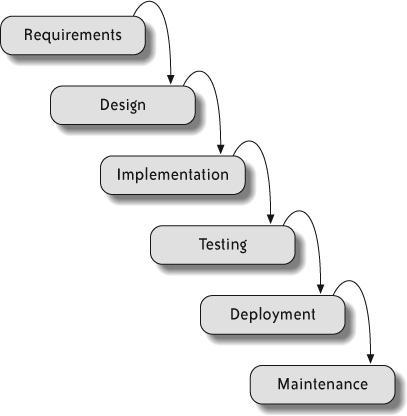
\includegraphics[scale=.86]{images/waterfall.png}
                \caption{SDLC, adapted from \cite{Hibbs2009} }
            \end{figure}
        \end{frame}
    
    \subsection{The Problem}
        \begin{frame}{What is Wrong?}
            \begin{itemize}
                \item Performance is difficult to measure
                \item Inconsistent
                \item Complicated
                \item Overwhelming
            \end{itemize}
        \end{frame}
    
\section{CRI}

    \subsection{CRI Overview}
        \begin{frame}{What is CRI?}
            \begin{displayquote}
                The \textit{Cumulative Result Indicator (CRI)} is an algorithm to provide a single 
                number score to measure the performance of an SDO. 
            \end{displayquote}
            \begin{enumerate}
                \item Quality
                \item Availability
                \item Satisfaction
                \item Schedule
                \item Requirements
            \end{enumerate}
        \end{frame} 
        
        \begin{frame}{CRI Attributes}
            \begin{itemize}
                \item The range of scores must have equal values above and below 0
                \item The minimum score must equate to the worst possible 
                    performance, however that is defined
                \item Similarly, the maximum score must equate to the best possible performance.  
                \item A score of 0 must be average (or expected) performance
                \item All individual elements must have the same scoring range
            \end{itemize}
        \end{frame} 
        
    \subsection{Quality}
        \begin{frame}{Quality Data}
        \end{frame} 
        \begin{frame}{Quality Baseline Function}
        \end{frame} 
        \begin{frame}{Quality Formula}
        \end{frame} 
    \subsection{Availability}
        \begin{frame}{Availability Data}
        \end{frame} 
        \begin{frame}{Availability Formula }
        \end{frame} 
    \subsection{Satisfaction}
        \begin{frame}{Satisfaction Data}
        \end{frame} 
        \begin{frame}{Satisfaction Formula }
        \end{frame} 
    \subsection{Schedule}
        \begin{frame}{Schedule Data}
        \end{frame} 
        \begin{frame}{Schedule Formula }
        \end{frame} 
    \subsection{Requirements}
        \begin{frame}{Requirements Data}
        \end{frame} 
        \begin{frame}{Requirements Formula }
        \end{frame} 
    \subsection{Overall}
        \begin{frame}{Overall Formula}
        \end{frame} 

    \subsection{Comparison}
        \begin{frame}{Requirements Data}
        \end{frame} 
    
    \subsection{Storage Framework}
        \begin{frame}{SDLC-AE}
            \begin{figure}[ht]
                \centering
                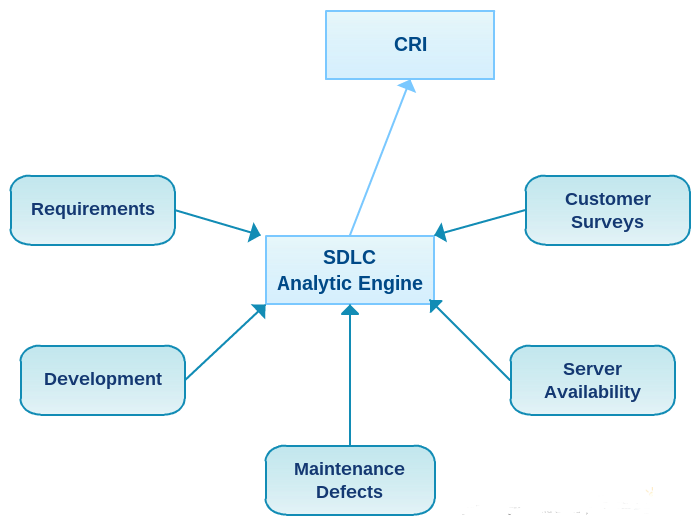
\includegraphics[scale=.5]{images/sdlcae.png}
            \end{figure}
        \end{frame}

\section{Case Study}
        \begin{frame}{Case Study Overview}
            \begin{itemize}
                \item SDO of a Large Financial Institution
                \item Data spans years 2008 - 2015
                \item $k = 100$
            \end{itemize}
        \end{frame}
    \subsection{Quality}
        \begin{frame}{CRI Quality Scores}
            \begin{figure}
                \centering
                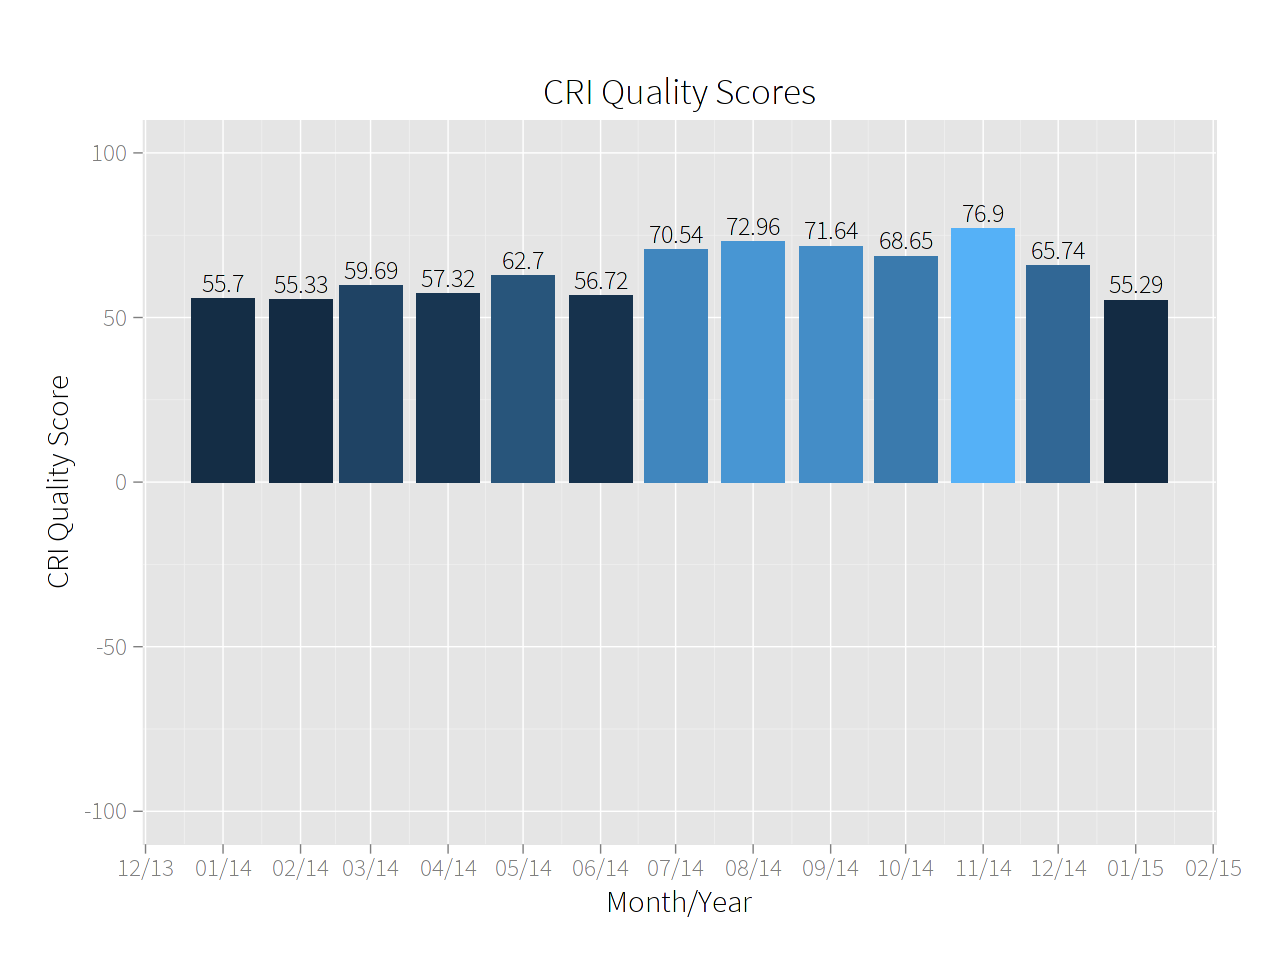
\includegraphics[scale=.23]{images/quality_scores.png}
            \end{figure}
        \end{frame}
    \subsection{Availability}
        \begin{frame}{CRI Availability Scores}
            \begin{figure}
                \centering
                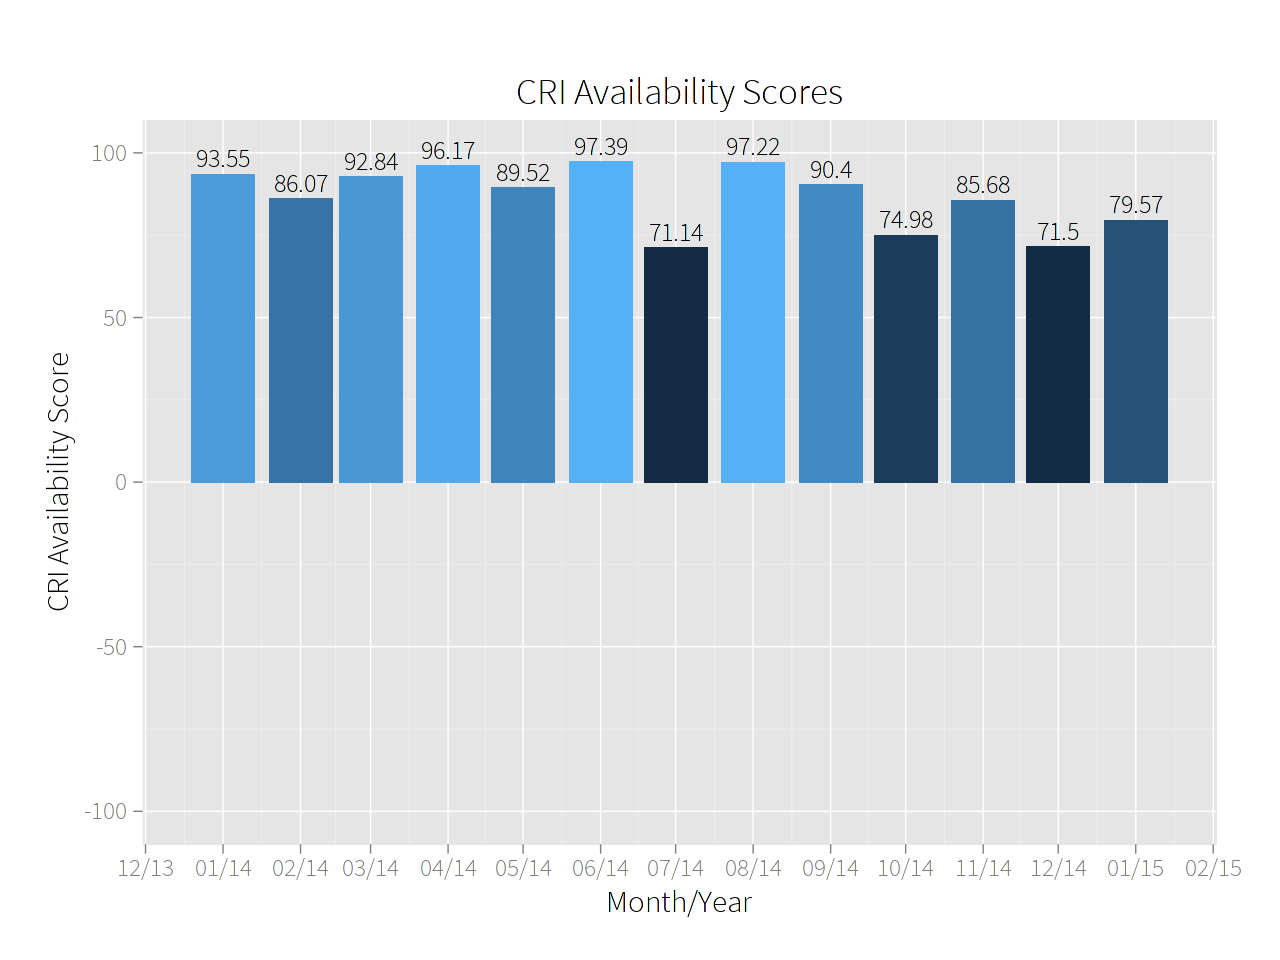
\includegraphics[scale=.23]{images/availability_scores.png}
            \end{figure}
        \end{frame}
    \subsection{Schedule}
        \begin{frame}{CRI Schedule Scores}
            \begin{figure}
                \centering
                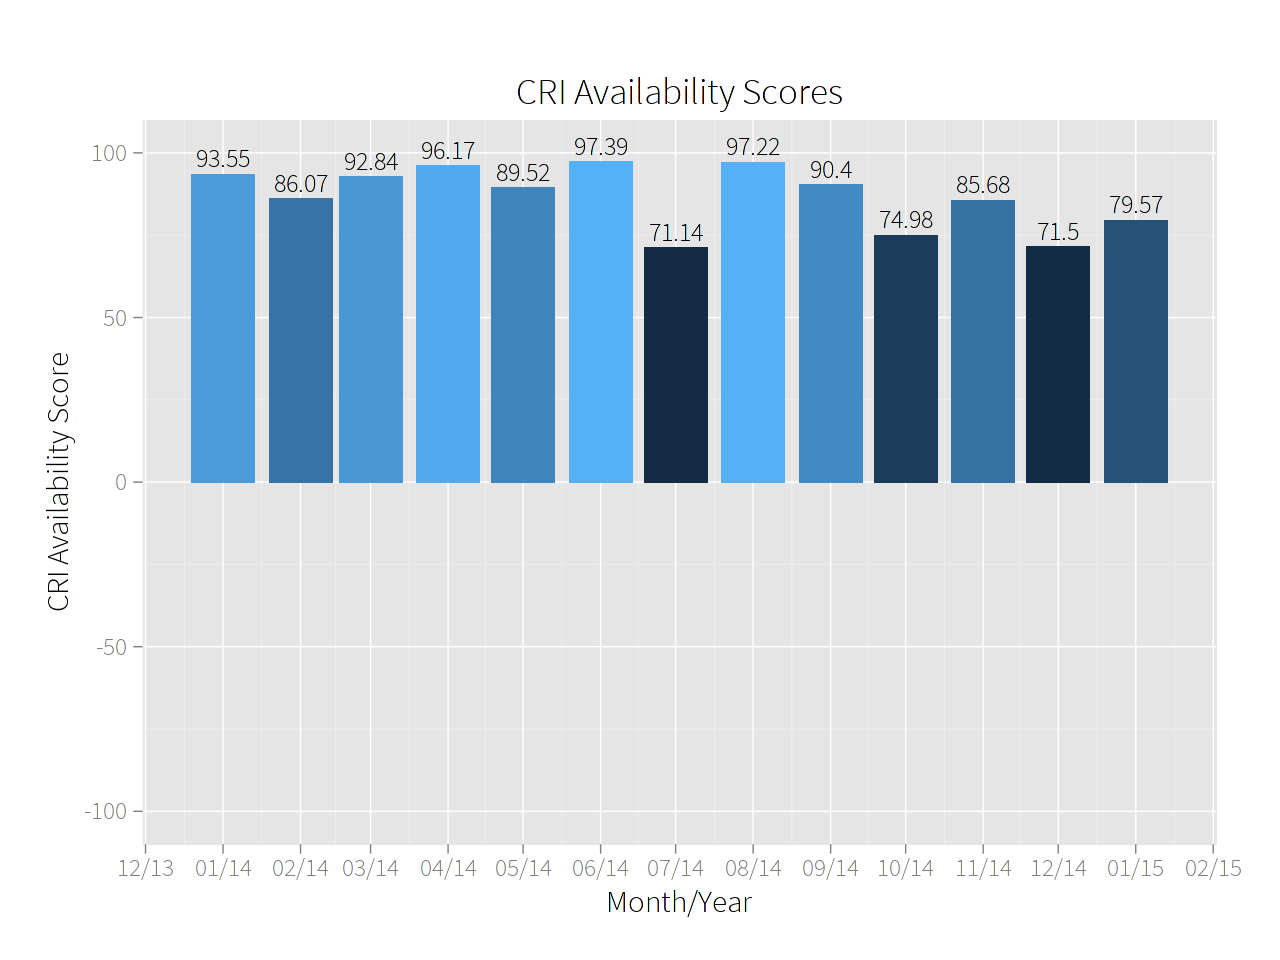
\includegraphics[scale=.23]{images/availability_scores.png}
            \end{figure}
        \end{frame}
    \subsection{Requirements}
        \begin{frame}{CRI Requirements Scores}
            \begin{figure}
                \centering
                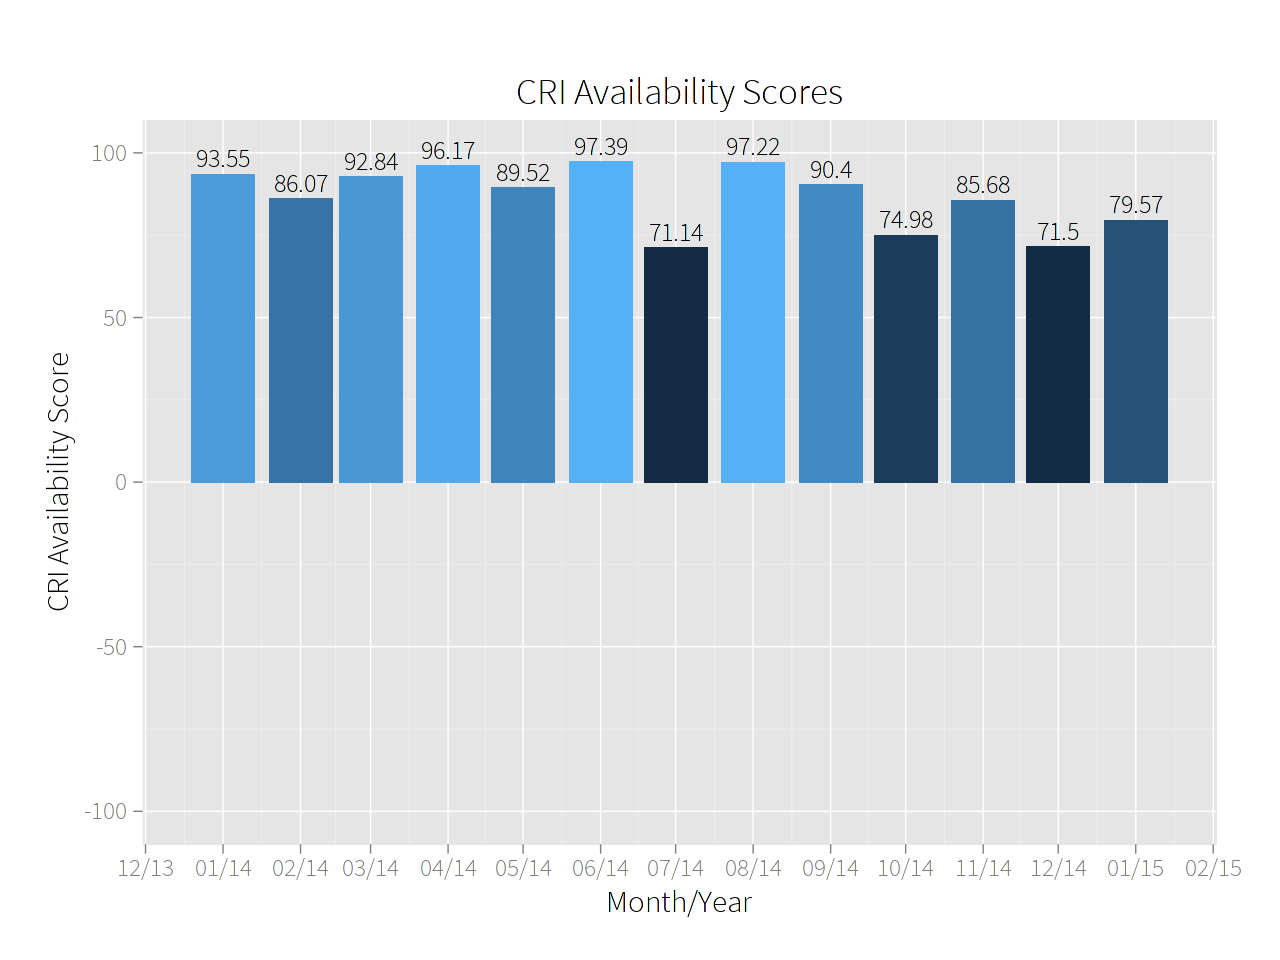
\includegraphics[scale=.23]{images/availability_scores.png}
            \end{figure}
        \end{frame}
    \subsection{Overall}
        \begin{frame}{CRI Availability Scores}
            \begin{figure}
                \centering
                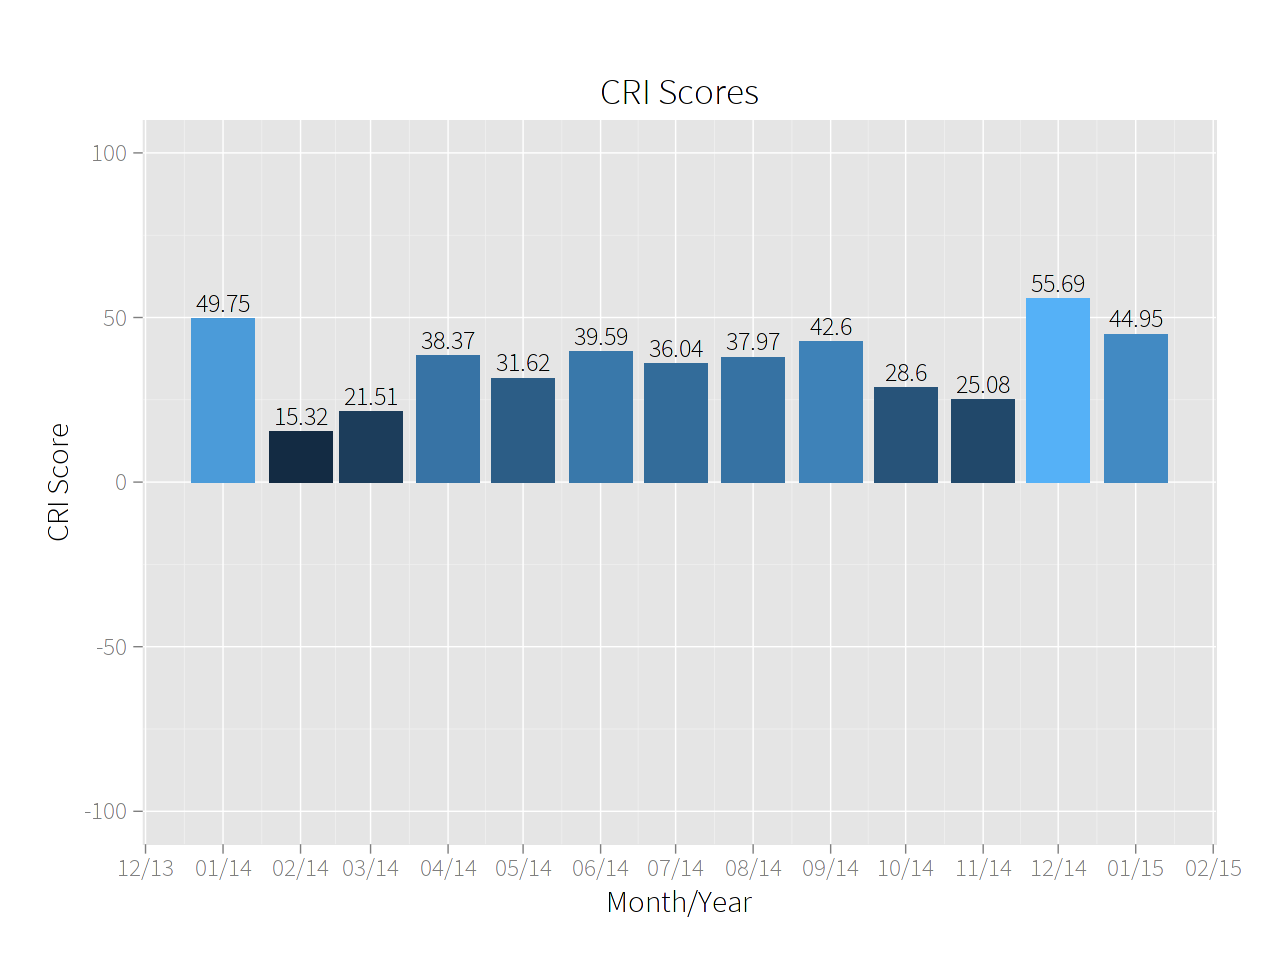
\includegraphics[scale=.23]{images/cri_scores.png}
            \end{figure}
        \end{frame}

\section{Conclusion}

    \subsection{Questions}
        \begin{frame}{Feedback}
            \center 
            Thanks for attending
            
            Questions / Thoughts
          
        \end{frame}

    \subsection{References}
        \begin{frame}{References}
            \bibliographystyle{acm}
            \bibliography{references}
          
        \end{frame}

\end{document}
